%
% koerperturm.tex -- Turm von Differentialkoerpererweiterungen
%
% Geschachtelte Rechtecke: Q(x) ⊂ F1 ⊂ F2 ⊂ ... ⊂ F_N, jede Stufe
% adjungiert Wurzeln, Logarithmen oder Exponentiale. Die Schachtelung
% ist die Inklusion.
%
\documentclass[tikz]{standalone}
\usepackage{amsmath}
\usepackage{amssymb}
\usepackage{times}
\usepackage{txfonts}
\definecolor{darkred}{rgb}{0.8,0,0}
\definecolor{darkblue}{rgb}{0,0,0.6}
\begin{document}
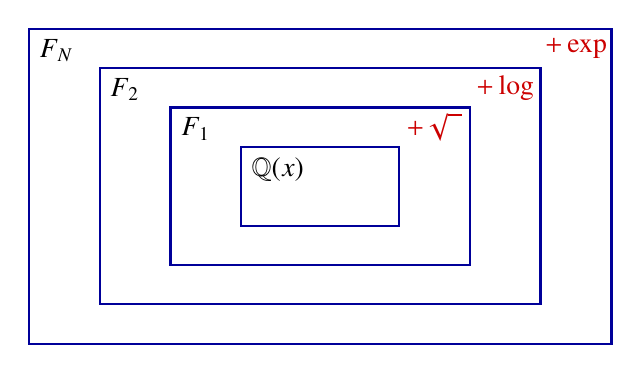
\begin{tikzpicture}[>=latex, thick]

% vier geschachtelte Rechtecke um denselben Mittelpunkt
\draw[darkblue] (-1.0,-0.5) rectangle (1.0,0.5);
\draw[darkblue] (-1.9,-1.0) rectangle (1.9,1.0);
\draw[darkblue] (-2.8,-1.5) rectangle (2.8,1.5);
\draw[darkblue] (-3.7,-2.0) rectangle (3.7,2.0);

% Koerpernamen in der linken oberen Ecke ihres Rechtecks
\node[anchor=north west] at (-1.0, 0.5) {$\mathbb{Q}(x)$};
\node[anchor=north west] at (-1.9, 1.0) {$F_1$};
\node[anchor=north west] at (-2.8, 1.5) {$F_2$};
\node[anchor=north west] at (-3.7, 2.0) {$F_N$};

% Erweiterungsschritte im Ring zwischen den Rechtecken, rechts oben
\node[darkred] at (1.45,0.75) {$+\sqrt{\phantom{x}}$};
\node[darkred] at (2.35,1.25) {$+\log$};
\node[darkred] at (3.25,1.75) {$+\exp$};

\end{tikzpicture}
\end{document}
